% Options for packages loaded elsewhere
\PassOptionsToPackage{unicode}{hyperref}
\PassOptionsToPackage{hyphens}{url}
%
\documentclass[
  11pt,
]{book}
\usepackage{amsmath,amssymb}
\usepackage{setspace}
\usepackage{iftex}
\ifPDFTeX
  \usepackage[T1]{fontenc}
  \usepackage[utf8]{inputenc}
  \usepackage{textcomp} % provide euro and other symbols
\else % if luatex or xetex
  \usepackage{unicode-math} % this also loads fontspec
  \defaultfontfeatures{Scale=MatchLowercase}
  \defaultfontfeatures[\rmfamily]{Ligatures=TeX,Scale=1}
\fi
\usepackage{lmodern}
\ifPDFTeX\else
  % xetex/luatex font selection
\fi
% Use upquote if available, for straight quotes in verbatim environments
\IfFileExists{upquote.sty}{\usepackage{upquote}}{}
\IfFileExists{microtype.sty}{% use microtype if available
  \usepackage[]{microtype}
  \UseMicrotypeSet[protrusion]{basicmath} % disable protrusion for tt fonts
}{}
\makeatletter
\@ifundefined{KOMAClassName}{% if non-KOMA class
  \IfFileExists{parskip.sty}{%
    \usepackage{parskip}
  }{% else
    \setlength{\parindent}{0pt}
    \setlength{\parskip}{6pt plus 2pt minus 1pt}}
}{% if KOMA class
  \KOMAoptions{parskip=half}}
\makeatother
\usepackage{xcolor}
\usepackage[left=4cm, right=3cm, top=2.5cm, bottom=2.5cm]{geometry}
\usepackage{longtable,booktabs,array}
\usepackage{calc} % for calculating minipage widths
% Correct order of tables after \paragraph or \subparagraph
\usepackage{etoolbox}
\makeatletter
\patchcmd\longtable{\par}{\if@noskipsec\mbox{}\fi\par}{}{}
\makeatother
% Allow footnotes in longtable head/foot
\IfFileExists{footnotehyper.sty}{\usepackage{footnotehyper}}{\usepackage{footnote}}
\makesavenoteenv{longtable}
\usepackage{graphicx}
\makeatletter
\newsavebox\pandoc@box
\newcommand*\pandocbounded[1]{% scales image to fit in text height/width
  \sbox\pandoc@box{#1}%
  \Gscale@div\@tempa{\textheight}{\dimexpr\ht\pandoc@box+\dp\pandoc@box\relax}%
  \Gscale@div\@tempb{\linewidth}{\wd\pandoc@box}%
  \ifdim\@tempb\p@<\@tempa\p@\let\@tempa\@tempb\fi% select the smaller of both
  \ifdim\@tempa\p@<\p@\scalebox{\@tempa}{\usebox\pandoc@box}%
  \else\usebox{\pandoc@box}%
  \fi%
}
% Set default figure placement to htbp
\def\fps@figure{htbp}
\makeatother
\setlength{\emergencystretch}{3em} % prevent overfull lines
\providecommand{\tightlist}{%
  \setlength{\itemsep}{0pt}\setlength{\parskip}{0pt}}
\setcounter{secnumdepth}{1}
\usepackage[]{natbib}
\bibliographystyle{apalike-es}
\usepackage{bookmark}
\IfFileExists{xurl.sty}{\usepackage{xurl}}{} % add URL line breaks if available
\urlstyle{same}
\hypersetup{
  pdftitle={Manual para organizar y analizar datos},
  pdfauthor={Salvador Mandujano Rodríguez},
  hidelinks,
  pdfcreator={LaTeX via pandoc}}

\title{Manual para organizar y analizar datos}
\author{Salvador Mandujano Rodríguez}
\date{September 11, 2025}

\begin{document}
\maketitle

{
\setcounter{tocdepth}{1}
\tableofcontents
}
\listoffigures
\listoftables
\setstretch{1.1}
\chapter*{Resumen}\label{resumen}
\addcontentsline{toc}{chapter}{Resumen}

El presente documento describe paso a paso el uso del paquete \texttt{RAI} desarrollado para calcular índices de abundancia relativa (RAI) a partir de una misma base de datos obtenidas durante el fototrampeo, empleando la plataforma de R. El paquete calcula el \texttt{RAI} de tres maneras: 1) de la forma tradicional donde se agrupan los datos y se obtiene un solo valor por especie, 2) considerando cada cámara como una répicla espacial lo que permite un análisis estadístico más robusto al estimar la variación del índice, y 3) como un modelo lineal generalizado (GLM) tipo regresión Poisson calibrando por el número de días por cámara. El paquete \texttt{RAI} tiene 12 funciones que generan tablas, figuras y análisis estadísticos. En este artículo se ejemplifica el uso de este paquete con un conjunto de datos de un estudio de foto-trampeo en la Reserva de Biósfera Tehuacán-Cuicatlán en Oaxaca, México. El paquete \texttt{RAI} está disponible libremente.

\emph{Palabras clave}: cámara-trampa, índices abundancias relativas, modelos, distribución naive, modelo lineal generalizado.

\pagebreak

\chapter{Introducción}\label{introducciuxf3n}

Los índices de abundancia relativa (IAR o también como RAI por sus siglas en inglés) tienen larga tradición en los estudios y monitoreo de fauna silvestre \citep{Delgado-Martinez2017}; particularmente, para especies raras y/o difíciles de detectar \citep{Raices2017}. Frecuentemente los RAI son usados como un indicador de la abundancia de la(s) especie(s) en el sitio de estudio \citep{effects2009}. Algunos RAI clásicos son los basados en las estaciones olfativas \citep{fegraus2011data}, conteo de aves en puntos por unidad de tiempo \citep{chao2014unifying}, conteo de nidos y madrigueras , conteo de huellas a lo largo de caminos, conteo de excrementos en parcelas \citep[\citet{chao2014unifying}]{chao2012coverage}, conteos de senderos \citep{hill1973diversity} y otros. En algunos casos, los índices son calibrados o convertidos a densidad poblacional, pero en la mayoría de los casos se emplean solo para un comparación relativa entre especies y para la misma especie en el mismo sitio de estudio o entre sitios \citep{hsieh2016inext}.

\section{Supuestos y limitantes del RAI}\label{supuestos-y-limitantes-del-rai}

El cálculo e interpretación del RAI es relativamente simple: basado únicamente en el valor del índice se determina cuales son las especies ``más o menos abundantes'' \citep{mccaffery1976deer}. Esta interpretación es cualitativa y subjetiva pero se reporta en la mayoría de los trabajos como una medida indirecta de la abundancia de cada especie \citep{sutherland2006ecological}. Sin embargo, esta comparación carece de rigor estadístico por lo que las conclusiones deben tomarse con mucho cuidado \citep{sutherland2006ecological}.

\section{Objetivos tesis}\label{objetivos-tesis}

En este artículo se presenta la aplicación del paquete \texttt{RAI} desarrollado para estimar índices de abundancia relativa para diferentes especies mediante el foto-trampeo (Mandujano, \emph{en revisión}). En particular, en este artículo se presenta paso a paso el procedimiento para estimar el RAI considerando tres modelos:

\begin{enumerate}
\def\labelenumi{\arabic{enumi})}
\tightlist
\item
  RAI tradicional o clásico;
\item
  RAI alternativo que permite estimar la variación considerando los datos de cada cámara como replicas, y luego compararlos estadísticamente, y
\item
  RAI como modelo lineal generalizado tipo Poisson.
\end{enumerate}

Para este fin, en este artículo se ejemplifica la aplicación de este paquete con un conjunto de datos obtenidos de 13 cámaras en una localidad de estudio en la Reserva de Biósfera Tehuacán-Cuicatlán en Oaxaca, México. Para detalles de este sitio se sugiere consultar los trabajos de Cruz-Jácome et al.~(2014), Mandujano et al.~(2016), y el blog \url{http://venadosrbtc.blogspot.com}.

\chapter{Marco teórico}\label{marco-teuxf3rico}

\section{Modelo clásico o general}\label{modelo-cluxe1sico-o-general}

La manera más frecuente para estimar el RAI de cada especie es agrupando la información obtenida en todas las cámaras (Fig.\ref{fig:f1}). Se define un periodo de tiempo en el cual se considera que las fotos de una misma especie son independientes. Una vez definido esto, se calcula el número de fotos independientes y se divide entre el total de tiempo de muestreo expresado como días o noche-trampa.

\begin{equation}
C \sim Poisson(\lambda p)
\label{eq:pois}
\end{equation}

donde: \(\lambda\) es el número total de registros fotográficos independientes de la \emph{i}-especie, \emph{p} es el esfuerzo de muestreo o número total de días. La Eq.\eqref{eq:pois} indica que si los conteos dependen de estos dos parámetros.

\begin{figure}

{\centering 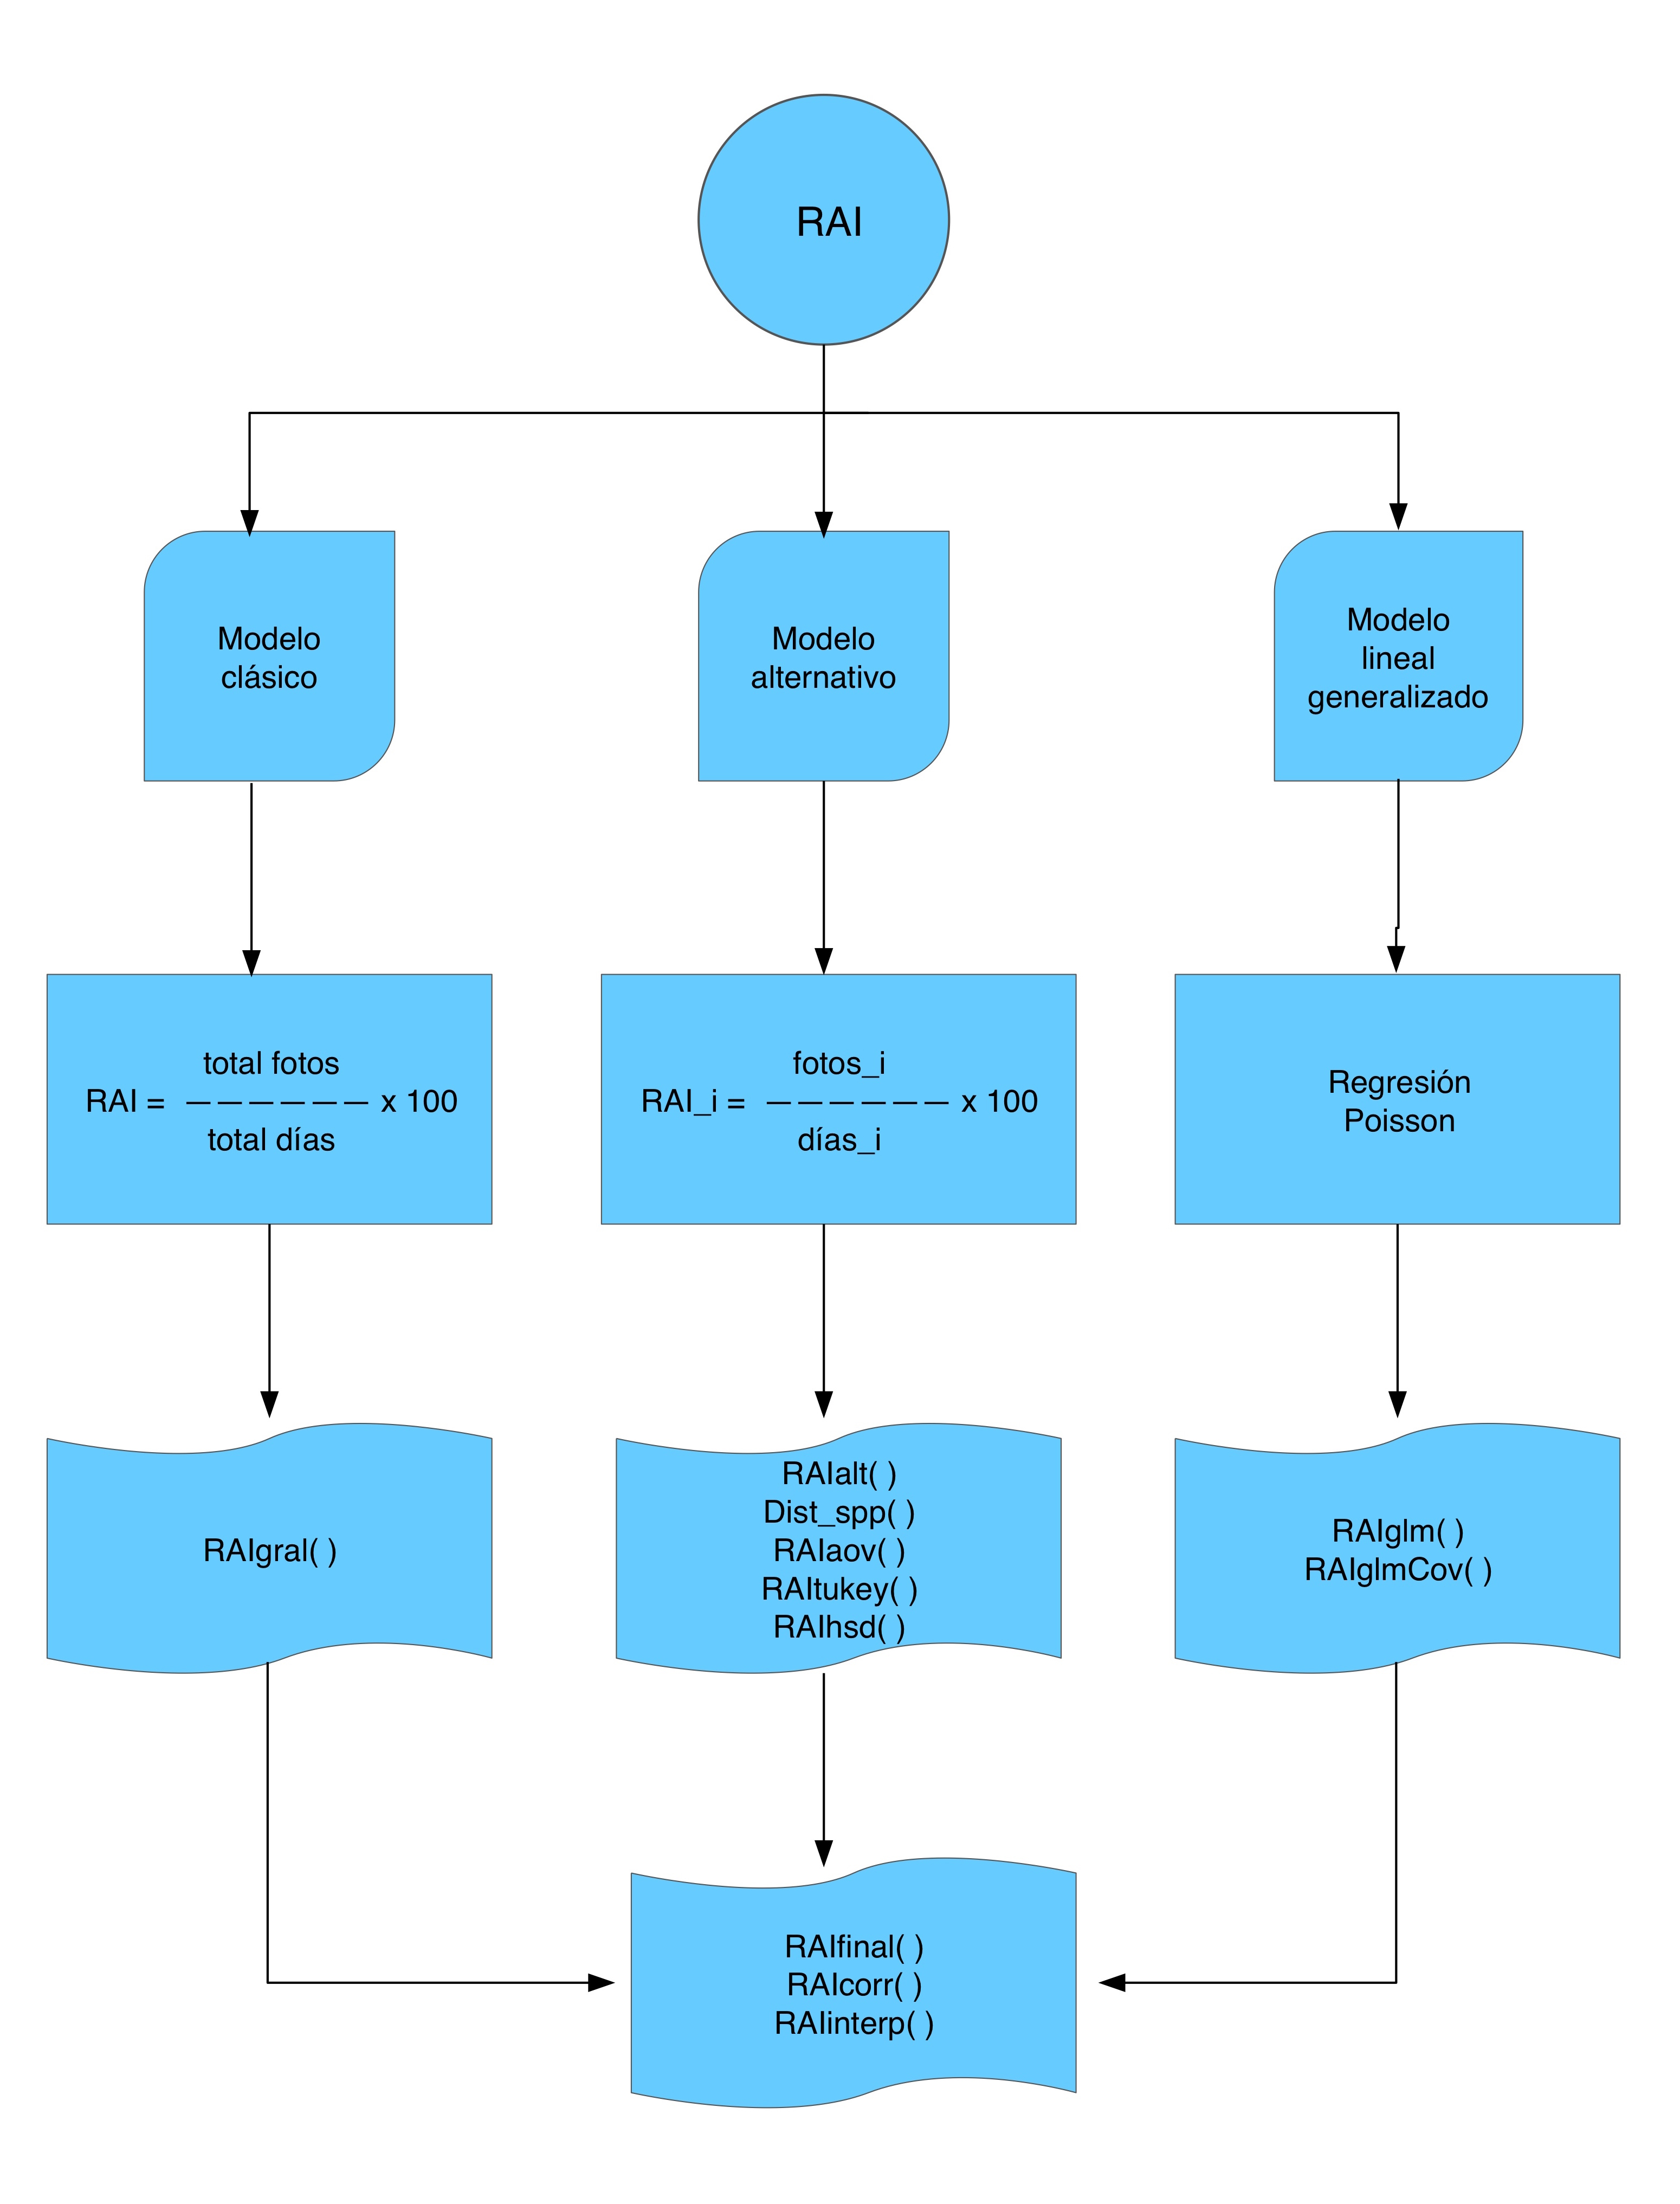
\includegraphics[width=0.75\linewidth]{figs/f1} 

}

\caption{Estructura del paquete RAI con las tres opciones de cálculo del índice de abundancia relativa y las 12 funciones asociadas.}\label{fig:f1}
\end{figure}

\section{Modelo lineal generalizado}\label{modelo-lineal-generalizado}

Otra manera completamente distinta de analizar los datos del foto-trampeo y calcular el RAI, es visualizarlo como un modelo lineal generalizado (GLM, por sus siglas en inglés de \emph{Generalized Lineal Model}). Los GLMs extienden el concepto del efecto lineal de las covariables para los casos donde las variables de respuesta o dependiente no se distribuyen de manera normal (Kéry y Royle 2016). Entonces el GLM se puede especificar como:

\begin{equation}
\begin{split}
n_{ij} \sim Poisson(Days_j \times \lambda_j) \\
log (Days_j \times \lambda_j) = \alpha_i + 1 \times log (Days_j) + \beta Covs 
\label{eq:glm}
\end{split}
\end{equation}

donde \emph{i} es la especie, \emph{j} el sitio, \(\lambda\) la abundancia, y \emph{Covs} las covariables. Un aspecto de la Eq.\eqref{eq:glm} es que cuando \(\beta Covs = 0\), entonces \(\alpha\) es lo mismo que la Eq.\eqref{eq:pois}.

\chapter{Métodos}\label{muxe9todos}

El estudio se realizó en la localidad de San Gabriel en la Reserva de Biosfera de Teahuácan-Cuicatlán, Oaxaca (Fig.\ref{fig:mapa}).

\begin{figure}

{\centering 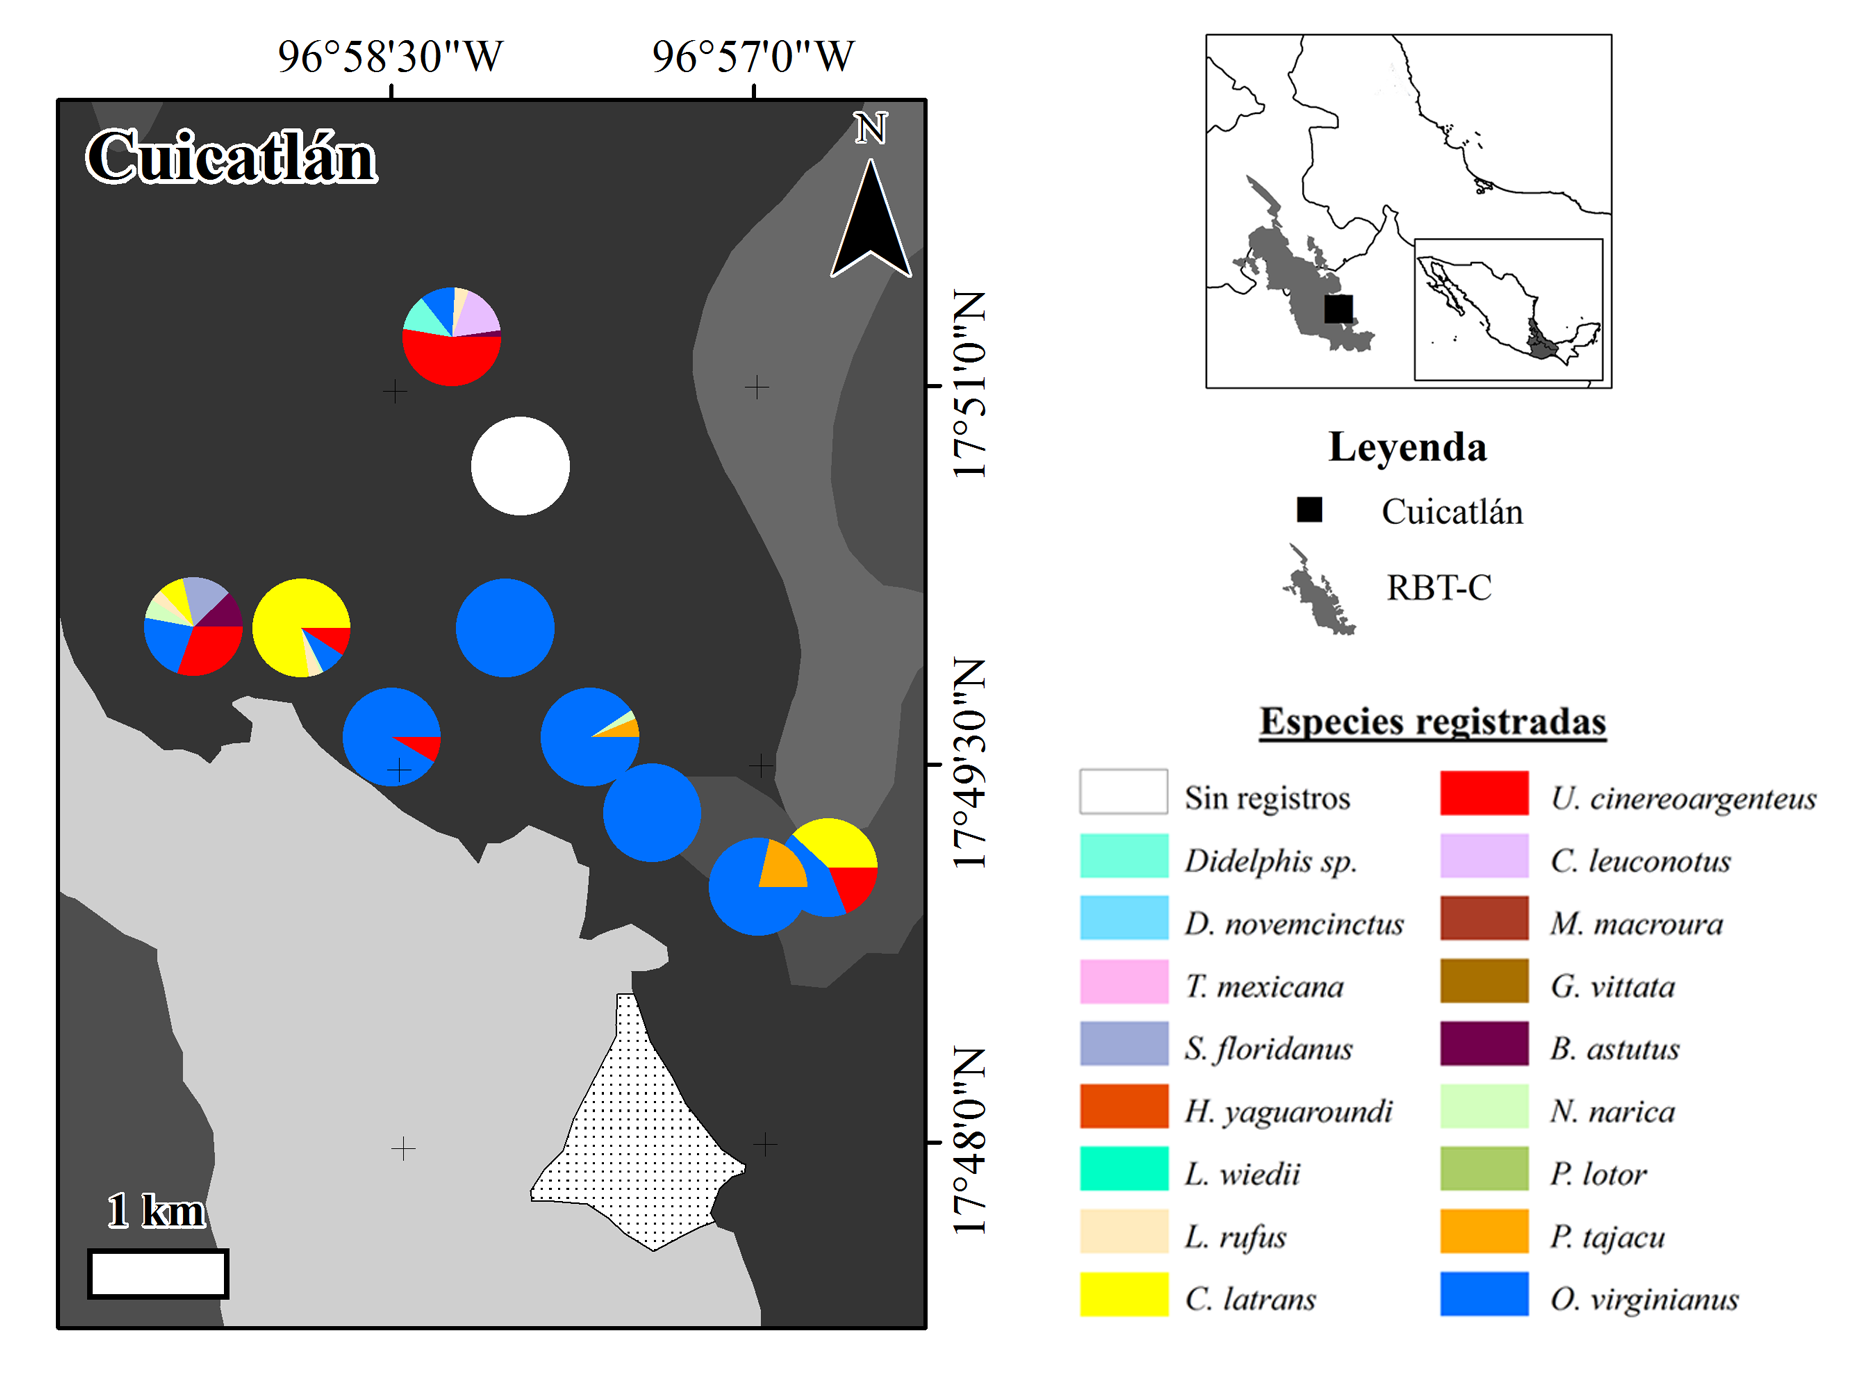
\includegraphics[width=2.48in]{figs/mapaRAI} 

}

\caption{Localización del área de estudio en la Reserva de Biósfera Tehuacán-Cuicatlán.}\label{fig:mapa}
\end{figure}

\section{Datos de campo}\label{datos-de-campo}

Se sugiere emplear Excel para capturar los datos del foto-trampeo. Esta tabla debe contener 4 columnas cada una con los siguientes nombres: \texttt{Camera}, \texttt{Species}, \texttt{Events} y \texttt{Effort}; que corresponden a la cámara-trampa, especie, número de fotos-independientes y número de días de muestreo, respectivamente. \textbf{Es muy importante que los nombres de las columnas sean exactamente como aquí se muestran de lo contrario el paquete no funcionará}. Una vez capturados los datos se deben guardar como archivo tipo \texttt{.csv}.

\section{Análisis}\label{anuxe1lisis}

Para ejemplificar el empleo de este paquete, se utilizará un conjunto de datos de 13 especies obtenidos de 13 cámaras en una localidad de estudio en la Reserva de Biósfera Tehuacán-Cuicatlán en Oaxaca, México. Para este fin, se sugiere descargar del sitio \url{http://RAI} los siguientes tres archivos: \texttt{mamiferos.csv}, \texttt{habitat.csv} y \texttt{pkgRAI\_1.R}. Los primeros dos son datos del ejemplo del foto-trampeo y covariables, respectivamente; mientras que el tercero es el paquete \texttt{RAI} el cual no requiere instalación. Sin embargo, para su correcta ejecuación se debe cargar primero empleando la función \texttt{source}.

\chapter{Resultados}\label{resultados}

\section{Datos}\label{datos}

Se sugiere generar un proyecto dentro de \texttt{RStudio} y albergar en el mismo estos tres archivos. Los proyectos son una manera muy sencilla y eficaz de organizar y almacener los resultados (Tabla \ref{tab:datos}). Por otro lado, era más frecuente para estimar el RAI de cada especie es agrupando la información obtenida en todas las cámaras. Se define un periodo de tiempo en el cual se considera que las fotos de una misma especie son independientes. Una vez definido esto, se calcula el número de fotos independientes y se divide entre el total de tiempo de muestreo expresado como días o noche-trampa. Por otro lado, era más frecuente para estimar el RAI de cada especie es agrupando la información obtenida en todas las cámaras. Se define un periodo de tiempo en el cual se considera que las fotos de una misma especie son independientes. Una vez definido esto, se calcula el número de fotos independientes y se divide entre el total de tiempo de muestreo expresado como días o noche-trampa

\begin{table}

\caption{\label{tab:datos}Datos del muestreo de mamíferos empleando cámaras.}
\centering
\begin{tabular}[t]{r|l|l|r|r|r|r|r}
\hline
Punto & Sitio & TVeg & Conteo & Densidad & HSI & Lluvia & Vacas\\
\hline
1 & ALM & Mat & 75 & 2.0 & 0.35 & 606 & 1\\
\hline
2 & CBL & BTC & 54 & 3.5 & 0.53 & 435 & 0\\
\hline
3 & CHI & BCo & 16 & 0.7 & 0.33 & 562 & 0\\
\hline
1 & CHL & Mat & 83 & 2.9 & 0.47 & 536 & 0\\
\hline
1 & CUI & Mat & 104 & 2.5 & 0.33 & 673 & 0\\
\hline
1 & FRO & Mat & 35 & 1.8 & 0.54 & 479 & 1\\
\hline
2 & IXC & BTC & 82 & 7.0 & 0.79 & 544 & 0\\
\hline
2 & JAL & BTC & 68 & 3.7 & 0.51 & 479 & 0\\
\hline
1 & JRY & Mat & 75 & 3.0 & 0.56 & 472 & 0\\
\hline
1 & LCU & Mat & 51 & 2.0 & 0.45 & 621 & 0\\
\hline
2 & MIA & BTC & 89 & 2.9 & 0.55 & 350 & 1\\
\hline
3 & PAP & BCo & 14 & 0.9 & 0.34 & 1332 & 1\\
\hline
3 & QUI & BCo & 16 & 0.9 & 0.30 & 676 & 1\\
\hline
3 & TEC & BCo & 54 & 1.9 & 0.64 & 564 & 1\\
\hline
2 & TEP & BTC & 65 & 3.1 & 0.53 & 713 & 0\\
\hline
2 & TPO & BTC & 105 & 3.8 & 0.60 & 905 & 0\\
\hline
3 & XOC & BCo & 40 & 1.5 & 0.56 & 613 & 1\\
\hline
3 & ZAR & BCo & 25 & 0.8 & 0.08 & 1257 & 1\\
\hline
\end{tabular}
\end{table}

\pagebreak

Por otro lado, era más frecuente para estimar el RAI de cada especie es agrupando la información obtenida en todas las cámaras (Tabla \ref{tab:anova}). Se define un periodo de tiempo en el cual se considera que las fotos de una misma especie son independientes. Una vez definido esto, se calcula el número de fotos independientes y se divide entre el total de tiempo de muestreo expresado como días o noche-trampa.

\begin{table}

\caption{\label{tab:anova}Análisis de varianza entre ...}
\centering
\begin{tabular}[t]{l|r|r|r|r|r}
\hline
X & Df & Sum.Sq & Mean.Sq & F.value & Pr..F.\\
\hline
Species & 15 & 5560.25 & 370.68331 & 7.591699 & 0\\
\hline
Residuals & 345 & 16845.47 & 48.82745 & NA & NA\\
\hline
\end{tabular}
\end{table}

\section{Relación entre variables}\label{relaciuxf3n-entre-variables}

En la Figura \ref{fig:corr} se muestra la relación\ldots tados.

\begin{figure}

{\centering 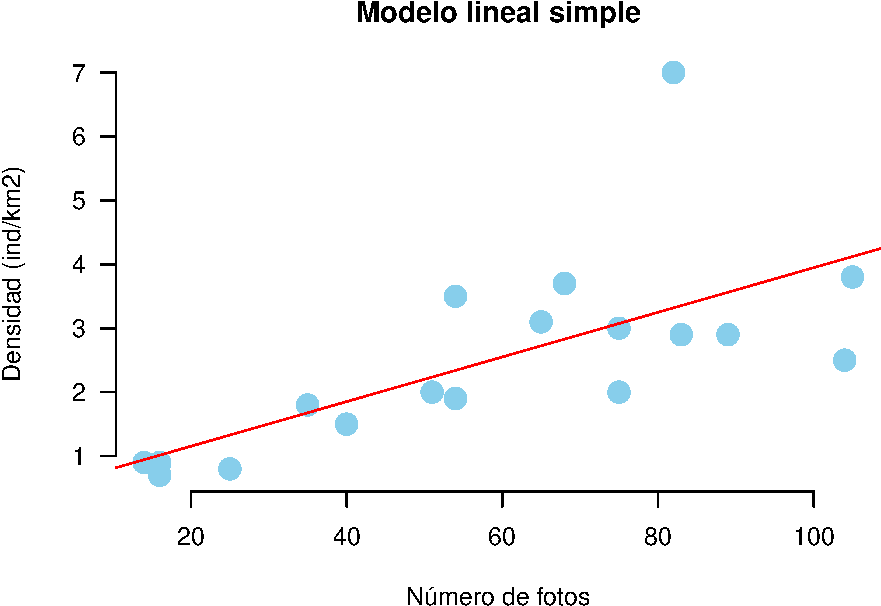
\includegraphics[width=0.8\linewidth]{Tesis_1_files/figure-latex/corr-1} 

}

\caption{Relación etc.}\label{fig:corr}
\end{figure}

\chapter{Discusión}\label{discusiuxf3n}

Los índices de abundancia relativa (IAR o también como RAI por sus siglas en inglés) tienen larga tradición en los estudios y monitoreo de fauna silvestre \citep{Delgado-Martinez2017}; particularmente, para especies raras y/o difíciles de detectar \citep{Raices2017}. Frecuentemente los RAI son usados como un indicador de la abundancia de la(s) especie(s) en el sitio de estudio \citep{effects2009}. Algunos RAI clásicos son los basados en las estaciones olfativas \citep{fegraus2011data}, conteo de aves en puntos por unidad de tiempo \citep{chao2014unifying}, conteo de nidos y madrigueras , conteo de huellas a lo largo de caminos, conteo de excrementos en parcelas \citep[\citet{chao2014unifying}]{chao2012coverage}, conteos de senderos \citep{hill1973diversity} y otros. En algunos casos, los índices son calibrados o convertidos a densidad poblacional, pero en la mayoría de los casos se emplean solo para un comparación relativa entre especies y para la misma especie en el mismo sitio de estudio o entre sitios \citep{hsieh2016inext}.

\renewcommand\bibname{Bibliografía}
  \bibliography{biblio.bib}

\end{document}
